\subsection{Simulationserweiterung}
\subsubsection{Steuerung}
\label{sec_waypoint}
Wie im Kapitel \ref{sec_auvSimGrundlage} Grundlagen beschrieben wird in der bestehenden Simulation ein \texttt{lane follower controller}, der eine Linie zwischen einem \textit{old\_waypoint} und einem \textit{new\_waypoint} bildet verwendet.
Die Schnittstelle zur Steuerung bildet also die Kombination aus den beiden Wegpunkten. Die Berechnung der Wegpunkte wird auf Basis des Polynoms aus dem Schätzverfahren generiert.\\
Zunächst wird die Position des AUVs durch die aktuelle Transformationsmatrix transformiert. Es wird der nächste Punkt auf dem Polynom zur transformierten Position des AUVs berechnet. Dieser Punkt dient als Zentrum für einen Kreis zur Bestimmung der Wegpunkte. Mithilfe der Kreisgleichung [Gleichung \ref{circEq}] werden die zwei Schnittpunkte des Polynoms mit dem Kreis berechnet. Da durch die Transformationsmatrix sichergestellt wird, dass das AUV in Richtung der $X-Achse$ fährt kann problemlos der Schnittpunkt mit höherem $x$ Wert als \textit{next\_waypoint} und dementsprechend der zweite als \textit{old\_waypoint} genommen werden. Es wird davon ausgegangen, dass bei einem solch kleinen Kreisradius (zwischen 5 und 10 Metern) nicht mehr als zwei Schnittpunkte zwischen Polynom und Kreis vorhanden sind. Sollte dies der Fall sein, wäre das Polynom viel zu stark gekrümmt, um noch verfolgt zu werden. Im Szenario dieser Arbeit gibt es auch keine Objekte, die eine solch starke Krümmung aufweisen.\\
Der letzte Schritt besteht aus der Transformation der Wegpunkte in das reale VRML-Koordinatensystem mithilfe der inversen Transformationsmatrix.
Das Verfahren ist in Abbildung \ref{wpCircle} grafisch dargestellt.

\begin{ownequation}[H]
\begin{equation}
0 = (X_{test}-Center_X)^2+(Y_{test}-Center_Y)^2 - r^2
\end{equation}
\caption{Kreisgleichung zum Test ob ein Punkt $X_{test},Y_{test}$ auf einem Kreis liegt}
\label{circEq}
\end{ownequation}

\begin{figure}[H]
\centering
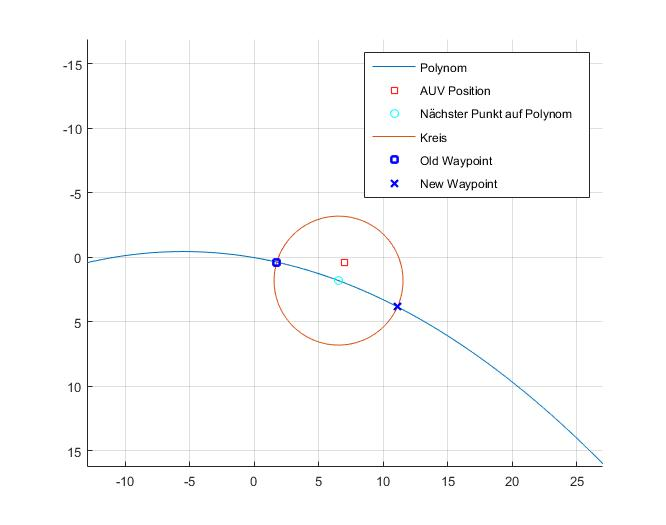
\includegraphics[scale=0.8]{waypointProvier.jpg}
\caption{Bestimmung der Wegpunkte}
\label{wpCircle}
\end{figure}
\subsubsection{Kamerabilder}
Da die Simulation in der Ursprünglichen Form noch sehr \textit{klinische} Bilder generierte mussten diese Bilder künstlich verschlechtert und die Sichtverhältnisse eingeschränkt werden, um realistische Eingangsbilder zu erzeugen. In Abbildung \ref{simPics} ist von links nach rechts ein ursprüngliches Kamerabild, ein verschlechtertes Bild und ein sehr stark verschlechtertes Bild zu sehen. Die Testläufe der Arbeit wurden mit dem Verschlechterungsgrad des mittleren Bildes durchgeführt. Die Objekterkennung wurde zudem noch mit Bildern, wie dem rechten Bild getestet.
\begin{figure}[H]
\begin{tabular}{ccc}
\subfloat[Ursprüngliches Bild]{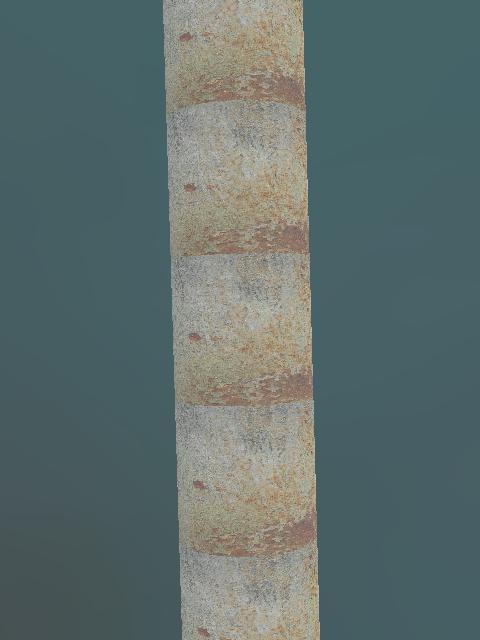
\includegraphics[scale=0.8,width=0.33\textwidth]{/imageProcessing/gradeOptimal.jpg}}&
\subfloat[Bild verschlechtert mit leichtem \textit{blur} und geringem Pixelrauschen]{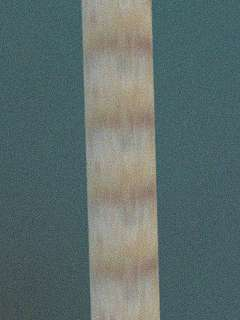
\includegraphics[scale=0.8,width=0.33\textwidth]{/imageProcessing/graeOk.jpg}}&
\subfloat[Bild verschlechtert mit starkem \textit{blur} und starkem Pixelrauschen]{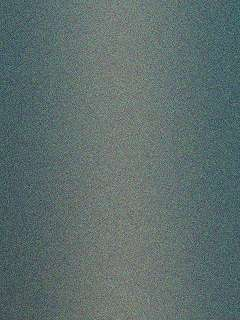
\includegraphics[scale=0.8,width=0.33\textwidth]{/imageProcessing/gradeschlecht.jpg}}\\
\subfloat[Sichtverhältnisse verschlechtert]{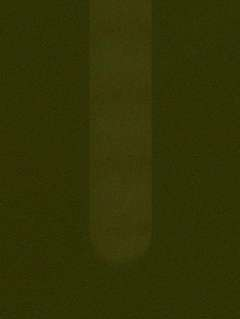
\includegraphics[scale=0.8,width=0.33\textwidth]{/imageProcessing/Prinzip/sim2,5Vis.jpg}}&
\subfloat[Sichtverhältnisse stark verschlechtert]{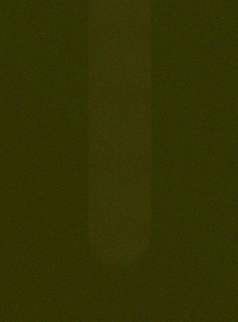
\includegraphics[scale=0.8,width=0.33\textwidth]{/imageProcessing//Prinzip/sim2Vis.jpg}}&
\subfloat[Sichtverhältnisse sehr stark verschlechtert und simulierte Reflexion des Wassers]{
\includegraphics[scale=0.8,width=0.33\textwidth]{/imageProcessing//Prinzip/sim2VisVielBlur.jpg}}
\end{tabular}
\caption{Simulationsbilder}
\label{simPics}
\end{figure}